\section{Radici di un'equazione (nonlineare)}
\footnote{PG 19-40, PDF lez6.} Il problema da risolvere è determinare
\begin{equation} \label{eq:radixEQ}
	x^*\in \mathbb R : f(x^*)=0,\quad f:\mathbb R\rightarrow \mathbb R.
\end{equation}

Per risolvere il problema è necessario determinare, se esiste/ono, la/e radice/i $x^*$ della funzione $f$, distinguendo i casi in base al numero di soluzioni del problema (\ref{eq:radixEQ}). Il problema (\ref{eq:radixEQ}):
\begin{enumerate} 
	\item ammette un numero finito di soluzioni (esempio: $f(x)=(x-1)(x^2-4)=(x-1)(x-2)(x+2)$);
	\item non ha soluzioni reali (esempio: $f(x)=e^x$);
	\item ammette infinite soluzioni reali (esempio: $f(x)=\sin(x)$, la quale si annulla in $\pi, 2\pi, \dots, k\pi, \dots,\, k\in\mathbb N$).
\end{enumerate}
Affinché il problema (\ref{eq:radixEQ}) sia risolvibile è necessario che ricada negli scenari 1. o 2. appena indicati.

\paragraph{Assunzione importante:} \textbf{in seguito sarà supposto che esista almeno una soluzione reale per (\ref{eq:radixEQ}) e che valga il Teorema degli zeri.} 

\begin{theorem}[degli zeri]
	Sia $f\colon I=[a,b]\rightarrow\mathbb R,\, f\in C([a,b]),\, f(a)f(b)< 0 \Rightarrow\exists x^* \in [a,b]:f(x^*)=0$.
\end{theorem}
\paragraph{N.B.:} È possibile fornire un intervallo di confidenza $[a,b]$ per la radice $x^*$. \textbf{La condizione} $\boldsymbol{f(a)f(b) < 0}$ \textbf{può essere verificata all'inizio dell'algoritmo che ricerca le radici.}

\addtocounter{footnote}{-1}
\footnotetext{L'implicazione è dovuta al Teorema degli zeri.}

\stepcounter{footnote}
\footnotetext{$f$ assume valori di segno opposto ai due estremi.}

\begin{figure}
	\centering
	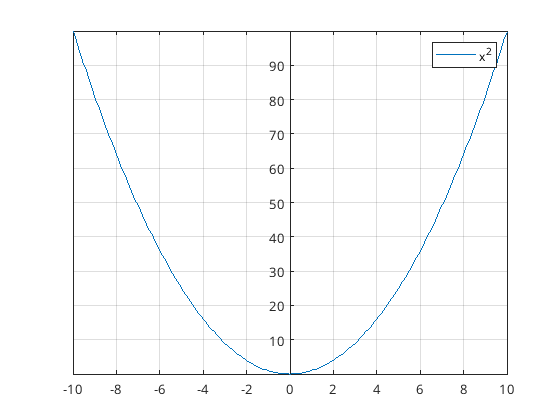
\includegraphics[width=0.5\textwidth]{immagini/Radix.png}
	\caption{\label{fig:SingleRadix}Grafico della radice della funzione $x^2$}
\end{figure}

\subsection{Metodo di bisezione}\footnote{PG. 19-22.} Data l'assunzione precedente, $[a,b]$ è un intervallo di confidenza per la radice $x^*$ di (\ref{eq:radixEQ}) (aumentandone così la precisione). Dovendo scegliere un punto nell'intervallo $[a,b]$, in modo tale che sia la migliore approssimazione della radice, è possibile porre $x^*\approx x_1=\frac{a+b}{2}$, ovvero selezionare il punto medio dell'intervallo.

Solo uno dei tre seguenti casi può verificarsi:
\begin{enumerate}
	\item $f(x_1)=0$, la soluzione è determinata ($x_1=x^*$);
	\item $f(a)f(x_1)<0$, il procedimento descritto può essere ripetuto sull'intervallo $[a, x_1]$ ($x^*\in[a, x_1]$);
	\item $f(x_1)f(b)<0$, il procedimento descritto può essere ripetuto sull'intervallo $[x_1, b]$ ($x^*\in[x_1, b]$).
\end{enumerate}

\begin{remark}
	È possibile osservare che nei casi 2. e 3. l'ampiezza dell'intervallo di confidenza si dimezza ad ogni passo perché sostituito, ad ogni passo, l'estremo opportuno.
\end{remark}

\begin{remark}
	Dati $[a_1,b_1]\equiv [a,b],\, x_1=\frac{a_1+b_1}{2}\Rightarrow x_n=\frac{a_n+b_n}{2}$, dove $x_n$ è l'approssimazione di $x^*$. Ulteriori chiarimenti sono forniti nella Sezione \ref{sec:critArresto}.
\end{remark}

È possibile che esistano più radici per la funzione $f$, un metodo iterativo come quello di bisezione ne approssima solamente una (vedere Figura \ref{fig:doubleRadix}).


\begin{example}
	Sia $p(x)=(x-1.1)^{20}(x-\pi)$, in Matlab $p(\pi)\approx 10^{-5}$. È possibile, in altri termini, ottenere il seguente risultato:
	\begin{lstlisting}[style=Matlab-editor]
		p = poly([1.1*ones(1,20) pi]);
		polyval(p,pi);
		ans = -5.521324170132402e-05
	\end{lstlisting}
\end{example}

\paragraph{Implementazione del metodo di bisezione:} Vedere Algoritmo \ref{alg:metodo_bisezione}.

\begin{figure}
	\centering
	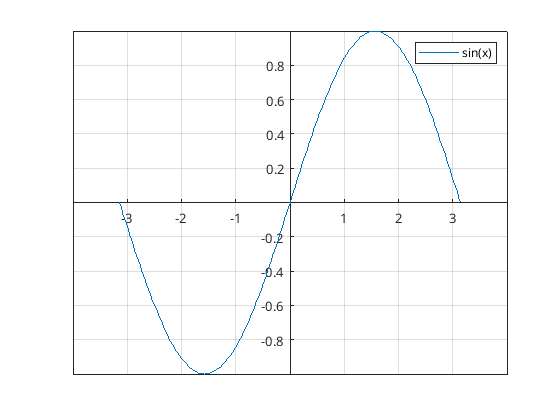
\includegraphics[width=0.5\textwidth]{immagini/tripleRadix.png}
	\caption{\label{fig:doubleRadix}Grafico della funzione con più radici $\sin{(x)}$}
\end{figure}

\subsection{Criterio di Arresto}\label{sec:critArresto}
Quando è possibile fermare la successione di approssimazioni $x_n$? Un possibile criterio d'arresto può essere $f(x_n)=0$. Questa condizione è improbabile che si verifichi, quindi inutilizzabile, perché è possibile arrivare alla radice $x^*$ solo quando $x^*=x_n$, quindi in un numero infinito di passi. Questo non è compatibile con un elaboratore in aritmetica finita, dove $f(x^*)=f(x_n)\neq 0$, a causa dell'aritmetica finita stessa.

Realisticamente è possibile richiedere che 
\begin{equation}\label{eq:x_n_leq_tolx}
	|x_n-x^*|\leq \boldsymbol{tolx},
\end{equation}
dove $\boldsymbol{tolx}$ è noto, in quanto scelto dall'utente e rappresenta il massimo errore (assoluto) che sarà commesso. Questa disuguaglianza è utile al fine di determinare se esiste un numero finito di iterazioni che permetta un livello di tolleranza dell'errore accettabile ($\boldsymbol{tolx}$).

\subsubsection{Criterio di arresto per il metodo di bisezione} Dato un intervallo di confidenza iniziale $[a,b]\equiv [a_1,b_1]$ e l'approssimazione iniziale $x_1=\frac{(a_1+b_1)}{2}$, allora, al passo $i-$esimo, sarà ottenuto l'intervallo di confidenza $[a_i,b_i]$ e l'approssimazione $x_i=\frac{(a_i+b_i)}{2}$. Al passo $n-$esimo sarà ottenuto l'intervallo di confidenza $[a_n,b_n]$ e l'approssimazione $x_n=\frac{(a_n+b_n)}{2}$.

\paragraph{In quanti passi è approssimata la radice $\boldsymbol{x^*}$?}
Per il metodo di bisezione è possibile affermare che
\begin{equation*}
	\begin{matrix}
		\text{Numero iterazione} & \text{Errore} & \text{Intervallo di confidenza}\\\\
		1 & |x_1-x^*| \leq \frac{b-a}{2} & [a,b] \\\\
		2 & |x_2-x^*|\leq \frac{x_1-a}{2}=\frac{b-a}{4}  & [a_2,b_2]\\\\
		\vdots & \vdots & \vdots \\\\
		i & |x_i-x^*|\leq\frac{b-a}{2^i} & [a_i,b_i]\\\\
		\vdots & \vdots & \vdots \\\\
		n & |x_n-x^*|\leq\frac{b-a}{2^n} & [a_n,b_n]
	\end{matrix}
\end{equation*}
dove $\boldsymbol{\frac{b-a}{2^i}}$ è \textbf{stima dell'errore} al passo $i$-esimo.

L'obbiettivo è determinare $n$ in modo tale $|x_n-x^*|\leq tolx$. Fermandosi all'iterazione $n$ allora 
\begin{equation*}
	|x_n-x^*|\leq\frac{b-a}{2^n}\leq tolx,
\end{equation*}
è soddisfatto $\frac{b-a}{2^n}\leq tolx$ e quindi:
\begin{equation*}
	\begin{matrix}
		&& |x_n-x^*| &\leq& \boldsymbol{tolx}\\
		&\overset{\footnotemark}{\Rightarrow}&\frac{b-a}{2^n}&\leq& tolx \\
		&\Rightarrow& 2^n&\leq&\frac{b-a}{tolx}\\
		&\Rightarrow& \boldsymbol n &\boldsymbol\geq&\left\lceil \log_{2}\left(\frac{b-a}{tolx}\right)\right\rceil&\overset{\footnotemark}{=}&\boldsymbol{\lceil \log_{2}(b-a)-\log_{2}(tolx)\rceil}&\boldsymbol\equiv& \boldsymbol{itmax}.
	\end{matrix}
\end{equation*}

\addtocounter{footnote}{-1}
\footnotetext{$n$ è scelto in modo tale che si verichi ciò che segue.}

\stepcounter{footnote}
\footnotetext{$\lceil\, \rceil$ significa arrotondamento all'intero successivo.}

\begin{definition}[Numero massimo di iterazioni (metodo bisezione)]\label{def:itmax_metodo_bisezione}
	Dato l'insieme $[a,b]$, il numero massimo di iterazioni per verificare la conzione (\ref{eq:x_n_leq_tolx}) con il metodo di bisezione è
	\begin{equation*}
		\boldsymbol{\lceil \log_{2}(b-a)-\log_{2}(tolx)\rceil \equiv itmax}
	\end{equation*}
\end{definition}

\paragraph{È possibile soddisfare $\boldsymbol{|x_n-x^*|\leq tolx}$ con meno di $\boldsymbol{itmax}$ passi:}
È possibile, per effettuare meno di $itmax$, approssimare $|x_i-x^*|$ come segue:
\footnote{Ricordando che di $f$ è ricercata la radice ovvero $x^*:f(x^*)=0$, allora è possibile quanto segue.}
\begin{equation*}
	\begin{matrix}
		f(x)&\overset{\footnotemark}{\equiv}& f(x^*)+f'(x^*)(x-x^*)&=&f'(x^*)(x-x^*)\\
		&\overset{\footnotemark}{\Rightarrow}&f(x_i)&\approx& f'(x^*)(x_i-x^*)\\
		&\overset{\footnotemark}{\Rightarrow}&\boldsymbol{|x_i-x^*|}&\boldsymbol\approx&\boldsymbol{\frac{|f(x_i)|}{|f'(x^*)|}}\\
		&\Rightarrow&\boldsymbol{|x_n-x^*|}&\boldsymbol\approx&\boldsymbol{\frac{|f(x_n)|}{|f'(x^*)|}}
	\end{matrix}
\end{equation*}

\addtocounter{footnote}{-2}
\footnotetext{Sviluppo di Taylor.}

\stepcounter{footnote}
\footnotetext{È ricercata $f(x_i)$, ovvero è effettuata la sostituzione $x=x_i$.}

\stepcounter{footnote}
\footnotetext{Essendo $|x_i-x^*|$ la quantità ricercata allora la conseguenza è logica.}

\noindent e quindi \textbf{è possibile utilizzare} $\boldsymbol{\frac{|f(x_i)|}{|f'(x^*)|}\leq tolx}$ \textbf{come criterio d'arresto} ($i=1,\hdots, n$). 

Al fine di utilizzare $f'(x^*)$ nel criterio di arresto, questa può essere approssimata, dato l'intervallo di confidenza $[a_i, b_i]$, come segue:
\begin{equation}\label{eq:approxf'}
	\boldsymbol{f'(x^*)\approx\frac{f(b_i)-f(a_i)}{b_i-a_i}=\frac{f(a_i+\overbrace{b_i-a_i}^{h})-f(a_i)}{\underbrace{b_i-a_i}_{h}}\rightarrow \lim_{i\to\infty}\frac{f(b_i)-f(a_i)}{b_i-a_i}}.
\end{equation}

\begin{remark}[Non ufficiale]
	Il costo computazionale dell'approssimazione $f'(x^*)$ calcolata come (\ref{eq:approxf'}) è nullo perché $f(a_i)$ e $f(b_i)$ sono già calcolati nel metodo di bisezione.
\end{remark}

Inoltre,
\begin{equation*}
	\frac{|f(x_i)|}{|f'(x^*)|}\leq tolx \iff |f(x_i)|\leq \boldsymbol{|f'(x^*)|\cdot tolx=tolf}(\rightarrow |f(x_i)|\leq tolf),
\end{equation*}
con ${tolf}$ quantità precisa [\footnotemark]. In altre parole: per avere $|x_n-x^*|\leq tolx$ occorre utilizzare una tolleranza $tolf\approx|f'(x^*)|\cdot tolx$.
\footnotetext{Se $tolf>>1$ (vedi Figura \ref{fig:f1(xStar)major1.jpg}), significa che $x_i$ è vicino a $x^*$ e ciò è un buon indicatore per determinare l'affidabilità legata all'errore.}

\begin{figure}
	\centering
	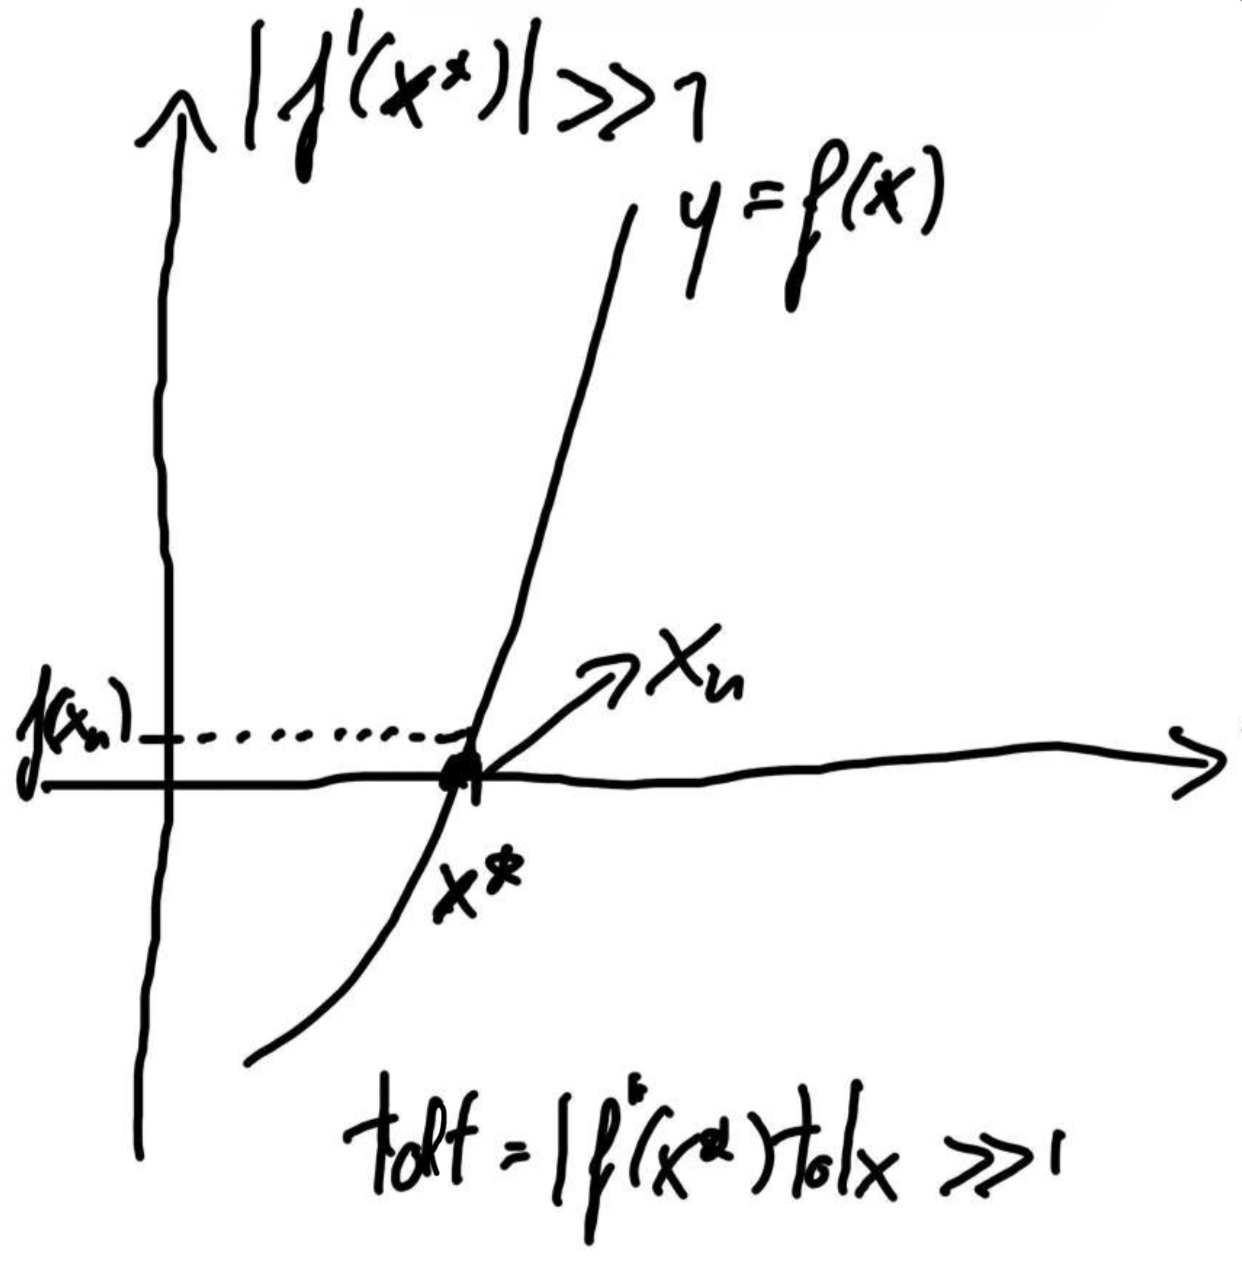
\includegraphics[width=0.5\textwidth]{immagini/f1(xStar)major1.jpg}
	\caption{\label{fig:f1(xStar)major1.jpg}$f'(x^*)>>1$}
\end{figure}
\begin{figure}
	\centering
	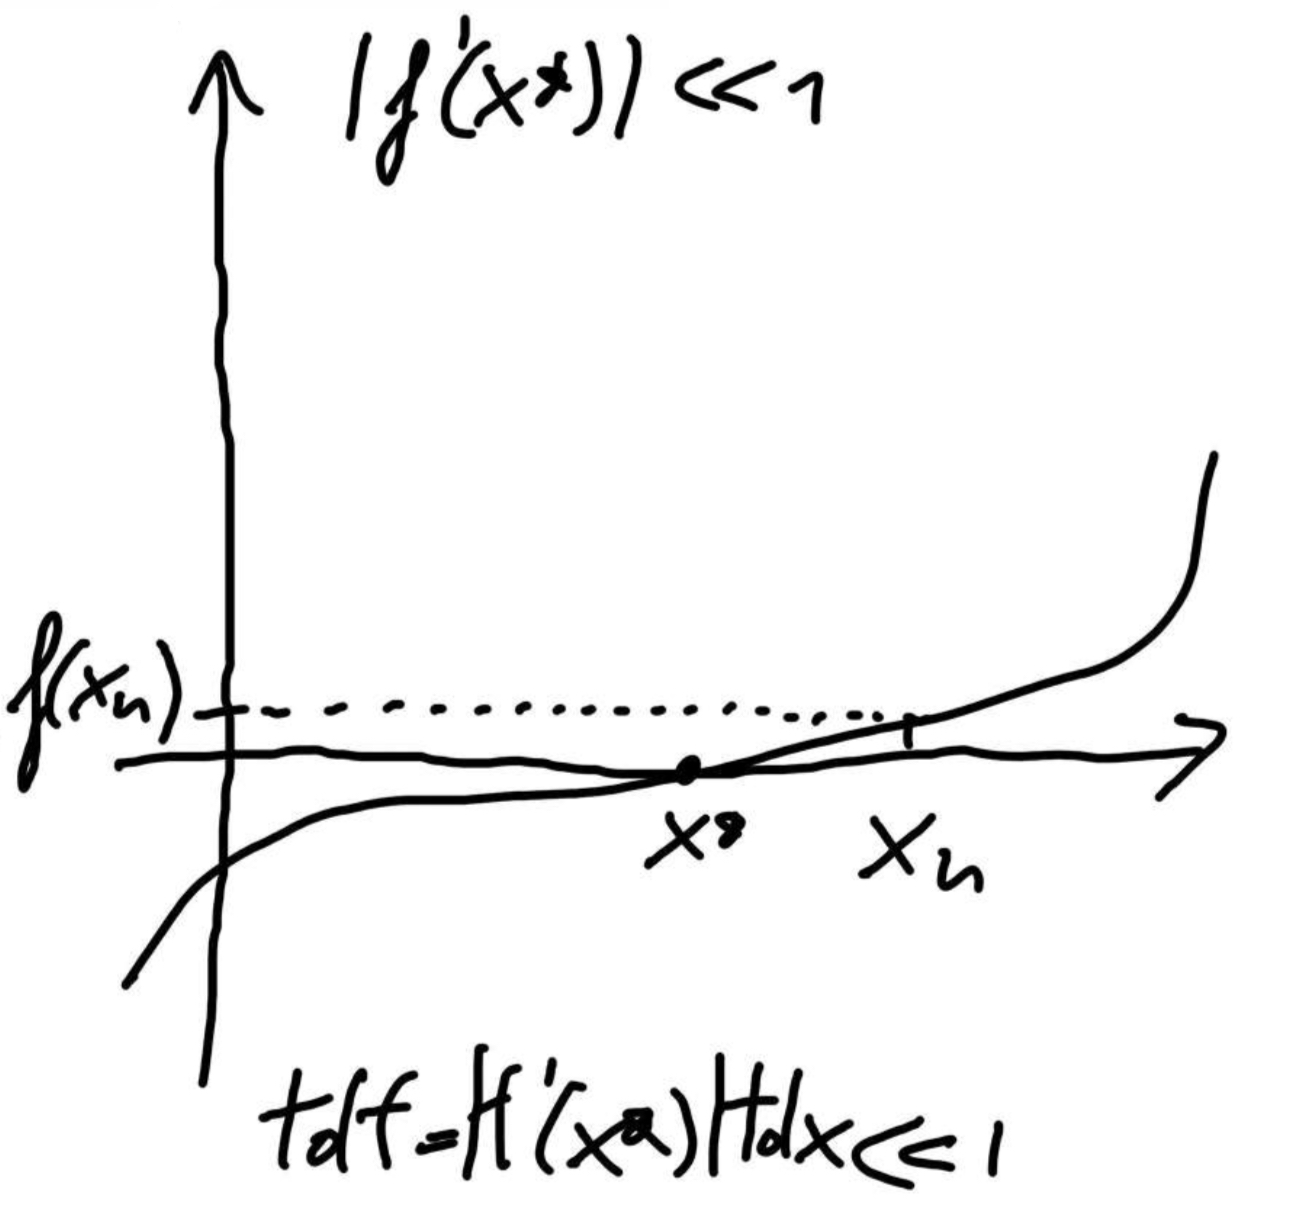
\includegraphics[width=0.5\textwidth]{immagini/f1(xStar)minor1.jpg}
	\caption{\label{fig:f1(xStar)minor1.jpg} $f'(x^*)<<1$}
\end{figure}

\subsubsection{Condizionamento di una radice}\footnote{PG 23, slide 6 PDF lez7.} L'analisi appena condotta per definire un criterio d'arresto più efficiente per il metodo di bisezione è altresì legata al condizionamento della radice $x^*$ e rimarrà valida anche per i metodi che saranno trattati successivamente.

\begin{definition}[Numero di condizionamento di una radice]\label{def:numero_condizionamento_radice}
	Sia $f$ ed $x^*$ la radice trovata. Il numero di condizionamento della radice $x^*$ è dato da
	\begin{equation}\label{eq:defK}
		\boldsymbol{\kappa =\frac{1}{|f'(x^*)|}.}
	\end{equation}
\end{definition}
Tale valore amplifica (di un fattore $\kappa$) l'errore $x_i-x^*$ commesso su $x^*$.

\begin{remark}[Non ufficiale]
	È possibile osservare che:
	\begin{itemize}
		\item se $|f'(x^*)|\approx 0\Rightarrow tolf\ll tolx\; \left(\frac{1}{|f'(x^*)|}\gg 1\right)$, $x^*$ è una radice malcondizionata;
		
		\item se $|f'(x^*)|\geq 1 \Rightarrow tolf\gg tolx\; \left(\frac{1}{|f'(x^*)|}\leq 1\right)$, $x^*$ è una radice bencondizionata.
	\end{itemize}
\end{remark}

\begin{example}[Condizionamento radice di un polinomio]\footnote{PG 25.}
	Nel caso del polinomio $p(x)=(x-1.1)^{20}(x-\pi)$ è ottenuta $p'(\pi)=(\pi-1.1)^{20}\approx 1.6\cdot 10^6$. Il numero di condizionamento vale $\kappa\approx 6\cdot 10^{-7}$ e quindi la radice $x^*=\pi$ è ben condizionata.
\end{example}

\begin{definition}[Errore (perturbazione) della radice]
	L'errore (perturbazione) sul risultato (di approssimazione della radice) è
	\begin{equation*}
		|x_n-x^*|\approx\frac{|f(x_n)|}{|f'(x^*)|}=\frac{1}{|f'(x^*)|}|f(x_n)|,
	\end{equation*}
	dove:
	\begin{itemize}
		\item $|f(x_n)|$ è la perturbazione rispetto al valore esatto $|f(x^*)|=0$,
		\item  $\frac{1}{|f'(x^*)|}$ il condizionamento della radice.
	\end{itemize}
\end{definition}

\paragraph{N.B.:} È necessario osservare che il condizionamento riguarda il problema e non il metodo numerico.

\begin{definition}[Radice con molteplicità $m$]\label{def:radice_molteplicita_m}
	\footnote{PG 25, slide 7 PDF lez 7.} $x^*$ è una radice del problema (\ref{eq:radixEQ}) ed ha molteplicità esatta $m\geq 1$, se è verificato quanto segue:
	\begin{equation*}
		f(x^*)=f'(x^*)=f''(x^*)=\hdots=f^{(m-1)}(x^*)=0,\, f^{(m)}(x^*)\neq 0.
	\end{equation*}
\end{definition}
Se $m=1$ allora $x^*$ si dice radice semplice, altrimenti (per $m\geq 2$) si dice multipla.

\paragraph{Il metodo di bisezione è malcondizionato con radici multiple:} Dalla Definizione precedente e dalla Definizione \ref{def:numero_condizionamento_radice} di condizionamento di una radice è possibile affermare che il problema della determinazione di radici multiple è \textbf{\underline{sempre} malcondizionato}, quindi non è consigliata l'applicazione del metodo di bisezione, in quanto il numero di condizionamento risulterebbe essere $\kappa=\infty$ (sarà ottenuto un risultato, la radice, non preciso).

\paragraph{Convergenza del metodo di bisezione:} Vedere Sezione \ref{ssec:convergenza_metodo_bisezione}.

\begin{algorithm}\caption{Implementazione ottimale del metodo di bisezione.}
	\label{alg:metodo_bisezione}
	\begin{lstlisting}[style=Matlab-editor]
		function x = bisezione(f, a, b) % da applicare controllo f(a)f(b)<0 (Teorema degli zeri)
		fa = feval(f, a);
		fb = feval(f, b);
		imax = ceil(log2(b-a) - log2(tolx));
		for i =  1 : imax
		x = (a + b)/2;
		fx = feval(f,x);
		f1x = abs((fb - fa)/(b - a));
		if abs(fx) <= tolx * f1x
		break
		elseif fa * fx < 0
		b = x;
		fb = fx;
		else
		a = x;
		fa = fx;
		end
		end
		return
	\end{lstlisting}
\end{algorithm}

\subsection{Convergenza di un metodo iterativo}\footnote{PG 26-28, slide 8-9 + 1-2 PDF lez7-8.} Lo scopo dell'argomento introdotto è quello di misurare l'errore di approssimazione della radice, quindi che il metodo iterativo sia corretto nel funzionamento. Ciò che sarà stabilito è la convergenza della successione alla radice.
\begin{definition}[Errore di approssimazione]
	Supposto di voler risolvere l'equazione (\ref{eq:radixEQ}) e sia $x_i$ l'approssimazione fornita al passo $i-$esimo, è possibile definire l'errore come
	\begin{equation}\label{eq:errore_metodo_iterativo}
		e_i:=x_i-x^*.
	\end{equation}
\end{definition} 

\begin{definition}[Metodo iterativo convergente]
	Un metodo iterativo è convergente s.se \begin{equation}\label{eq:limite_errore_metodo_convergente}
		\lim_{i\to\infty}{e_i}=0.
	\end{equation}
\end{definition}

\subsection{Ordine di Convergenza di un metodo iterativo}
Il passo successivo alla convergenza è stabilire la velocità computazionale del metodo (quanto velocemente $x_n$ si avvicina a $x^*$? Quanti calcoli servono?). Per questo è necessaria l'introduzione di \textbf{Definizione \ref{def:ordine_convergenza_metodo_iterativo}} di ordine di convergenza e \textbf{Osservazione \ref{rem:limOrdConv}.}
\begin{definition}[\textbf{Ordine di convergenza} di un metodo iterativo] \label{def:ordine_convergenza_metodo_iterativo}
	Se un metodo iterativo ha $p\in\mathbb R^+$ come valore più grande per cui \begin{equation}\label{eq:limOrdConv}
		\lim_{i\to\infty}{\frac{|e_{i+1}|}{|e_i|^p}}=c<\infty,
	\end{equation}
	allora tale metodo ha \textbf{ordine di convergenza} $\boldsymbol p$, con \textbf{costante asintotica dell'errore} pari a $\boldsymbol c$.
\end{definition}

\begin{remark}
	Se $e_i<1 \Rightarrow |e_i|^p$ è sempre più piccolo al crescere di $p$.
\end{remark}

\begin{remark}\label{rem:limOrdConv}
	Per $i$ sufficientemente grande, nel caso di convergenza lineare ($p=1$), è ottenuto (data (\ref{eq:limOrdConv})):
	\begin{equation*}
		\frac{|e_{i+1}|}{|e_i|^p}\approx c \Rightarrow |e_{i+1}|\approx c|e_i|^p.
	\end{equation*}
\end{remark}

\begin{remark}\label{rem:metodo_lineare_convergente}
	Un \textbf{metodo lineare} ($p=1$) è \textbf{convergente s.se} $\boldsymbol{0\leq c<1}$.
\end{remark}

\paragraph{Perché l'Osservazione \ref{rem:metodo_lineare_convergente} vale?} Dato $|e_{i+1}|\approx c|e_i|^p$ allora, se $p=1$ $|e_{i+1}|\approx c|e_i|\Rightarrow |e_{i+k}|\approx c^k|e_{i-k}|\Rightarrow |e_i|\approx c^i|e_0|$ quindi
\begin{equation*}
	\underset{i\to\infty}{\lim}|e_i|=\underset{i\to\infty}{\lim}{c^i|e_0|}\iff c<1.
\end{equation*}

Più è elevato l'ordine di un metodo convergente, più le approssimazioni generate dal metodo convergono verso la radice $x^*$. Questo è accentuato nel prossimo esempio.

\begin{example}
	\footnote{PG 27, slide 1 PDF lez8.} Considerati 2 metodi iterativi convergenti alla stessa radice $x^*$, con ordine di convergenza rispettivamente $p=1$ e $p=2$, entrambi con costante $c=0.1$, se per entrambi $e_0=0.1$, allora
	\begin{center}
		\begin{tabular}{ |c|c|c|c| } 
			\hline
			$i$ & $p=1$ & $p=2$ \\
			\hline
			0 & 0.1 & 0.1 \\ 
			1 & $c|e_0|^1=10^{-2}$ & $c|e_0|^2=10^{-3}$ \\ 
			2 & $c|e_1|^1=10^{-3}$ & $c|e_1|^2=10^{-7}$\\
			3 & $c|e_2|^1=10^{-4}$ & $c|e_2|^2=10^{-15}$\\
			4 & $c|e_3|^1=10^{-5}$ & $c|e_3|^2=10^{-31}$\\
			\hline
		\end{tabular}
	\end{center}
	
	È possibile osservare come la tabella sia ottenuta dall'applicazione della Definizione \ref{def:ordine_convergenza_metodo_iterativo} e che $e_i=c|e_{i-1}|^1,\, \forall i=1,\hdots , n$ (dove, nella tabella, $n=4$).
\end{example}

\subsubsection{Metodo di bisezione}\label{ssec:convergenza_metodo_bisezione}
\begin{remark}(Convergenza metodo di bisezione)
	Il metodo di bisezione è sempre convergente (convergenza globale): 
	\begin{equation*}
		|e_i|=|x_i-x^*|\leq \frac{b-a}{2^i}\Rightarrow \boldsymbol{0\leq \lim_{i\to\infty}|e_i|\leq \lim_{i\to\infty}{\frac{b-a}{2^i}=0}\Rightarrow \lim_{i\to\infty}{e_i}=0.}
	\end{equation*}
\end{remark}

\noindent Inoltre, \textbf{il metodo di bisezione ha ordine di convergenza assimilabile a $\boldsymbol{p=1}$ e costante asintotica dell'errore $\boldsymbol{c=\frac{1}{2}}$}, ovvero \textbf{converge linearmente} \footnotemark. Questo è dovuto a $\underset{{i\to\infty}}{\lim}{\frac{|e_{i+1}|}{|e_i|}}=\frac{1}{2}$, utilizzando la stima assegnata al metodo di bisezione $|e_i|\leq\frac{b-a}{2^i}$.

\footnotetext{Quindi il metodo di bisezione converge $R-$linearmente (informazione non richiesta).}

\subsection{Metodo di Newton}\label{ssec:metodo_newton}
\footnote{Slide 3-8, 1-2 PDF 8,11 PDF 9,10.}
Il metodo di Newton è un metodo di approssimazione della radice con ordine migliore del metodo di bisezione. Questo metodo si basa su un'approssimazione lineare della funzione a partire dalla soluzione approssimata corrente, ovvero: supposto di conoscere un'approssimazione $y$ della funzione, allora il sistema generale per determinare $x^*$ tale che $f(x^*)=0$ è
\begin{equation*}
	\begin{cases}
		y = f(x),\\
		y = 0,
	\end{cases}
\end{equation*}
dal quale, attraverso l'utilizzo della retta tangente al grafico di $f$ nel punto $(x_0,f(x_0))$
\begin{equation}\label{eq:retta_tangente_in_0}
	\begin{cases}
		y = f(x_0) + f'(x_0)(x-x_0), \\
		y = 0,
	\end{cases}
\end{equation}
è ricavata, tramite calcoli intermedi (\footnotemark), l'approssimazione (definita dall'approssimazione di tale retta con l'asse delle ascisse)
\begin{equation*}
	x_1=x_0-\frac{f(x_0)}{f'(x_0)},
\end{equation*}
la quale è definita per $f'(x_0)\neq 0$, con $x_0$ approssimazione iniziale di $x^*$. Reiterando per $i$ passi successivi, è possibile ottenere l'espressione funzionale del metodo di Newton:
\begin{equation}\label{eq:approxNewton}
	x_{i+1}=x_i-\frac{f(x_i)}{f'(x_i)}, \quad i=0,1,2,\hdots
\end{equation}

\footnotetext{Da (\ref{eq:retta_tangente_in_0}) $y=0\Rightarrow\frac{f(x_0)}{f'(x_0)}+\cancel{f'(x_0)}(x-x_0)=0\Rightarrow x-x_0=-\frac{f(x_0)}{x_0}\Rightarrow x=x_0-\frac{f(x_0)}{x_0}.$}

\begin{figure}
	\centering
	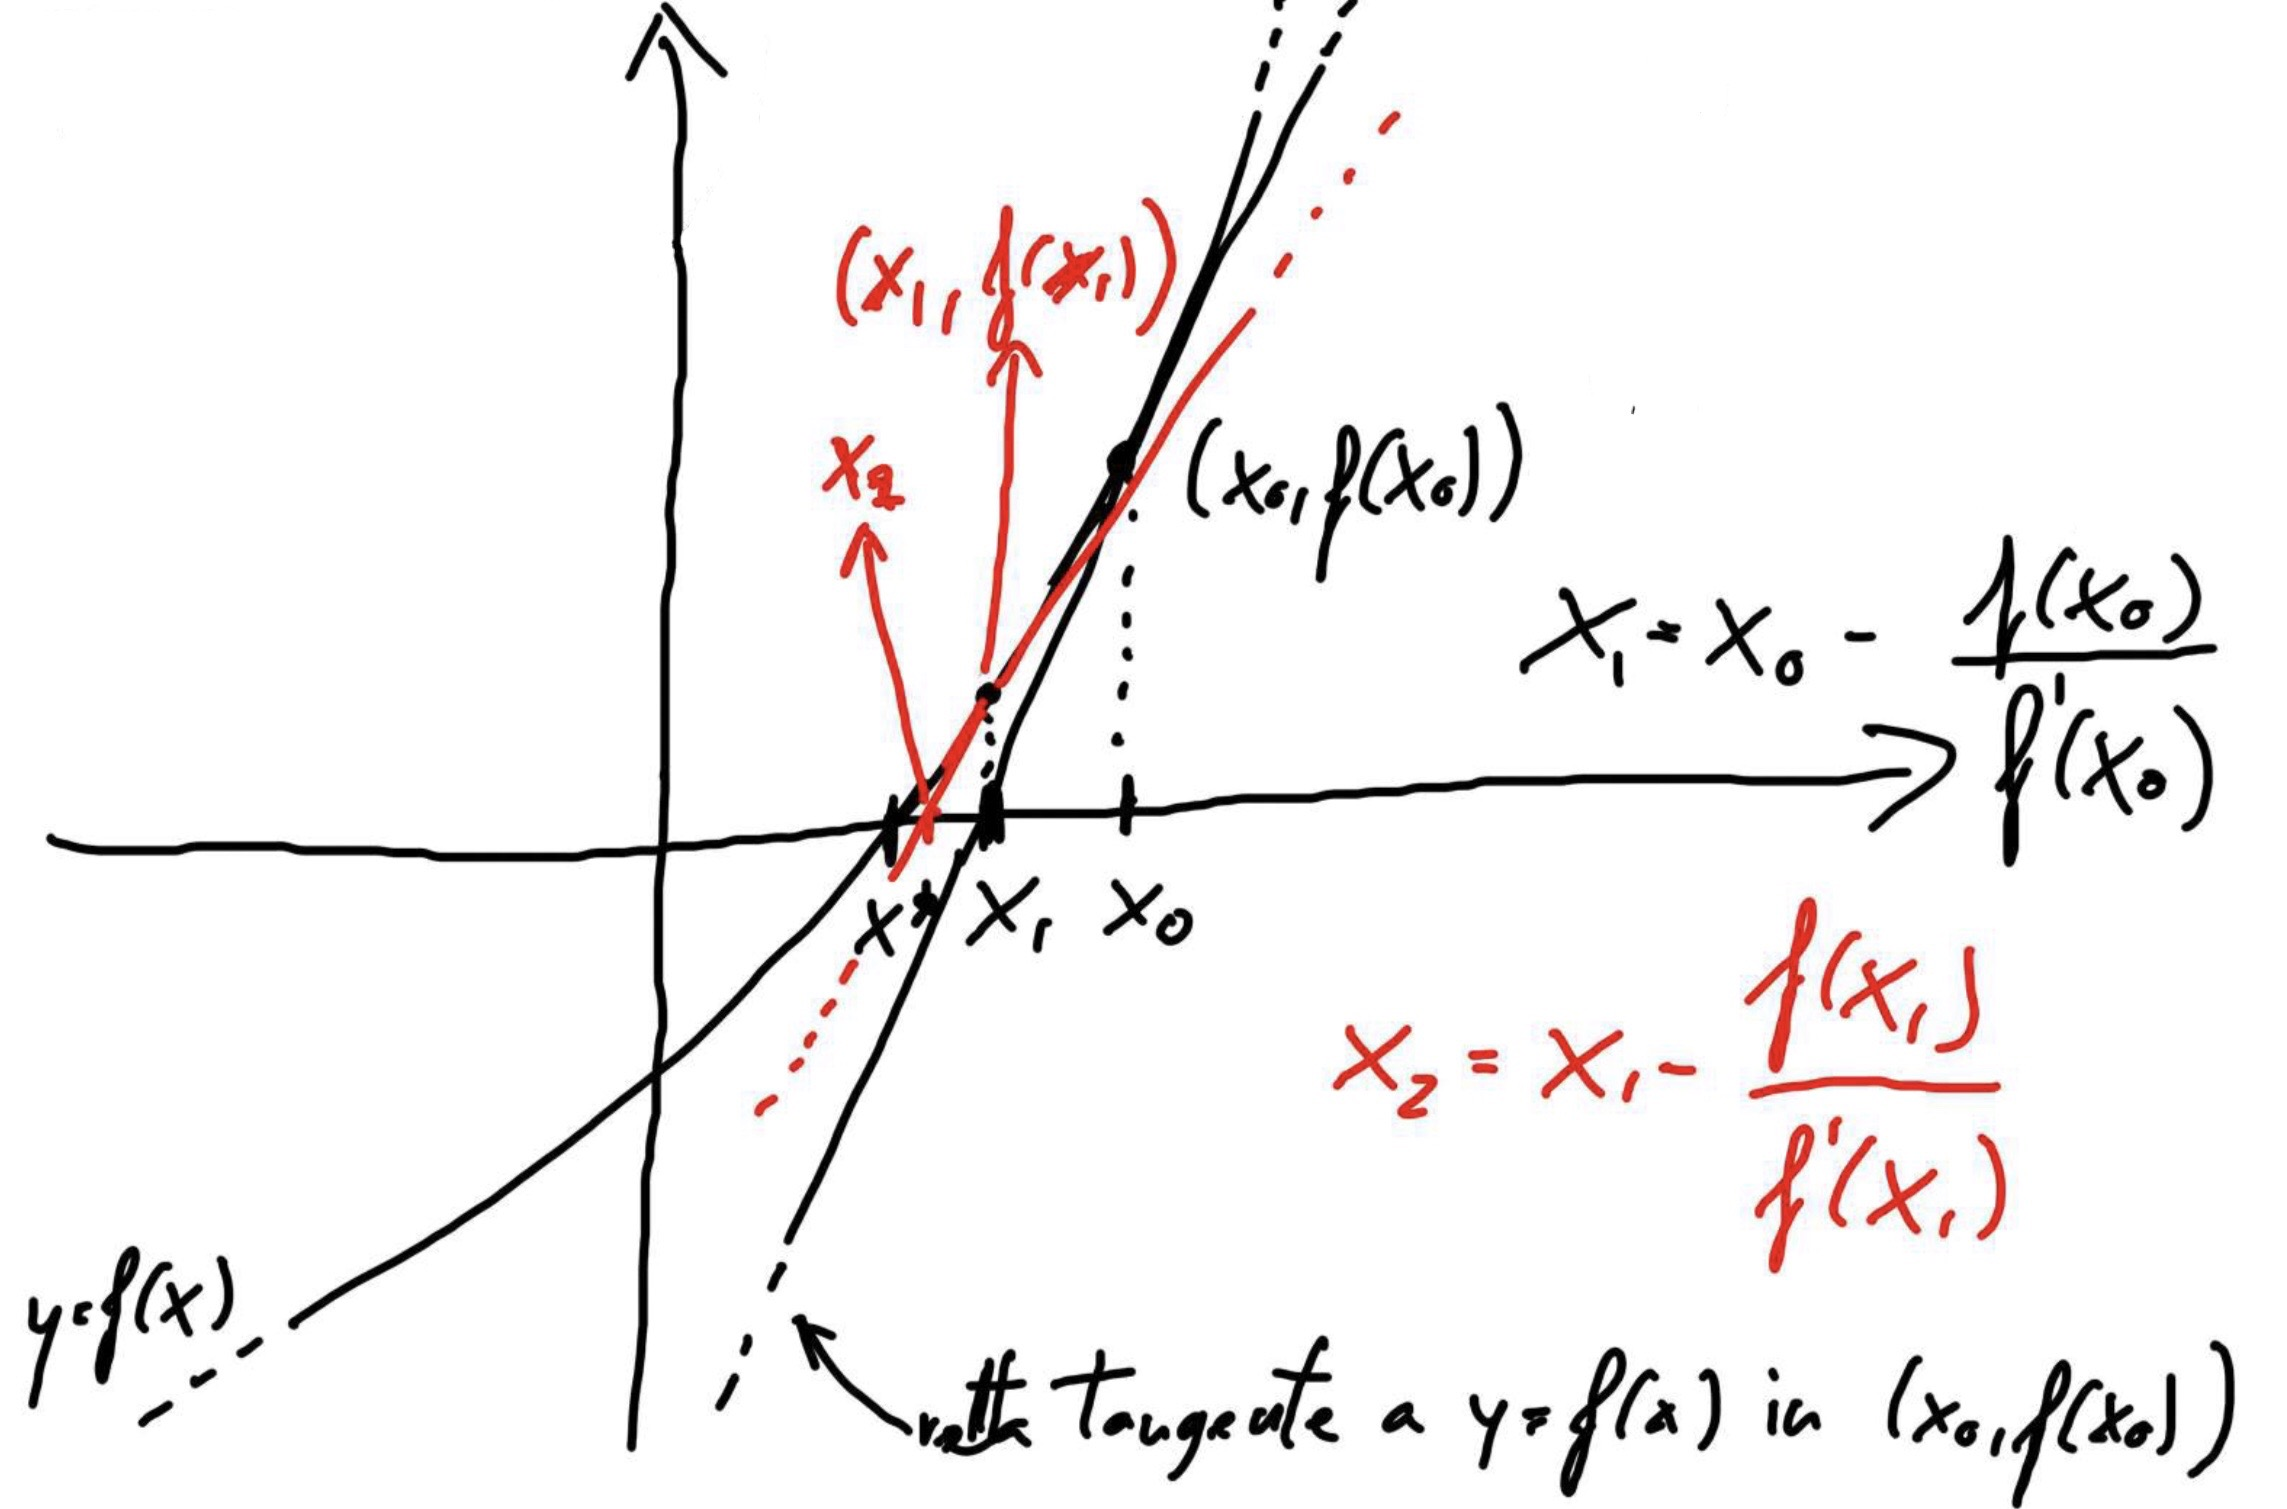
\includegraphics[width=0.5\textwidth]{immagini/GraficoRettaTangNewton.jpg}
	\label{fig:grafico_retta_tangente_metodo_newton}
	\caption{Grafico $y=f(x)$ con relative approssimazioni ottenute tramite Newton (è ricercata l'intersezione).}
\end{figure}

Più passi vengono calcolati, più $x_i$ si avvicina a $x^*$.

\paragraph{Osservazioni sul metodo:} La soluzione al problema (\ref{eq:radixEQ}) è ottenuta risolvendo \gls{equazioni lineari}. Nel caso in cui $f(x)$ sia una \gls{funzione lineare} allora il metodo di Newton fornisce la soluzione in un solo passo.

\paragraph{Costo computazionale:}È possibile osservare che il metodo di Newton ha un costo per iterazione di 2 valutazioni funzionali (il metodo di bisezione ne richiede una): è necessario calcolare $f(x)$ ed $f'(x)$, in quanto ad ogni passo/iterazione cambia l'input ($x_0, x_1, x_2, \hdots$).
Inoltre, mentre il metodo di bisezione richiede solo la continuità della funzione $f$, per il metodo di Newton è richiesto che $f$ sia, oltre che continua, derivabile (ovvero $f\in C^{(2)}$).
Il costo computazionale maggiore e maggiori requisiti del metodo, rispetto al metodo di bisezione, sono compensati dall'elevato ordine di convergenza del metodo.

\begin{theorem}[\textbf{Metodo di Newton converge quadraticamente}, nome non ufficiale]\label{th:metodo_newton_converge_quadraticamente}
	Se $f(x)$ è sufficientemente regolare, \textbf{il metodo di Newton converge quadraticamente} (ovvero con ordine $p=2$) \textbf{verso radici semplici} \footnote{Ovvero radici di molteplicità 1, le quali sono definite come $x^*:f(x^*)=0,\, f'(x^*)\neq 0$.}.
\end{theorem}
\begin{proof}
	Assunto che $f\in C^{(2)}$ in un intorno della radice $x^*$, preso un opportuno $\xi_i$ (non noto) compreso fra $x^*$ e $x_i$, tramite lo sviluppo di Taylor di ordine 2 centrato in $x_i$
	\begin{equation*}
		f(x)=f(x_i)+f'(x_i)(x-x_i)+\frac{f''(\xi_i)}{2}(x-x_i)^2, \quad \xi_i \text{ compreso fra }x,x_i,
	\end{equation*}
	è valutata $f$ tramite lo sviluppo di Taylor centrato in $x^*$
	\begin{equation*}
		\begin{matrix}
			0 &=& f(x^*)\\
			&=& f(x_i)+f'(x_i)(x^*-x_i)+\frac{f''(\xi_i)}{2}(x^*-x_i)^2 \\
			&\overset{\footnotemark}{=}& f'(x_i)\left[\frac{f(x_i)}{f'(x_i)}-x_i+x^*\right]+\frac{f''(\xi_i)}{2}(x^*-x_i)^2 \\
			&\overset{\footnotemark}{=}&f'(x_i)(-x_{i+1}+x^*)+\frac{f''(\xi_i)}{2}(x^*-x_i)^2\\
			&\overset{\footnotemark}{=}&-f'(x_i)e_{i+1}+\frac{f''(\xi_i)}{2}e_i^2 &\rightarrow&\frac{f''(\xi_i)}{2}e_i^2 &=& -f'(x_i)e_{i+1}\\
			&&&\overset{\footnotemark}{\Rightarrow}& \frac{|e_{i+1}|}{|e_i^2|} &=& \frac{1}{2}\frac{|f''(\xi_i)|}{|f'(x_i)|}, && x^*<\xi_i<x_i.
		\end{matrix}
	\end{equation*}
	\addtocounter{footnote}{-3}
	\footnotetext{Raccolto $f'(x_i)$ perché interessante la q.tà $\frac{f(x_i)}{f'(x_i)}-x_i$ (ovvero $x_{i+1}$ cambiato di segno).}
	
	\stepcounter{footnote}
	\footnotetext{Sostiuzione di $\frac{f(x_i)}{f'(x_i)}-x_i$ con $-x_{i+1}$.}
	
	\stepcounter{footnote}
	\footnotetext{Sostituzione $x^*-x_{i+1}=-e_{i+1}$ e $x^*-x_i=-e_i$.}
	
	\stepcounter{footnote}
	\footnotetext{L'obbiettivo è valutare quanto segue.}
	
	\noindent Allora, supponendo che il metodo converga (ovvero che $\lim_{i\rightarrow+\infty}x_i=x^*$): 
	\begin{equation*}
		\lim_{i\to\infty}{\frac{|e_{i+1}|}{|e_i|^2}}=\lim_{i\to\infty}{\frac{1}{2}\frac{f''(\xi_i)}{f'(x_i)}}\overset{\footnotemark}{=}\frac{1}{2}\frac{f''\left(\underset{i\to\infty}{\lim}\xi_i\right)}{f'\left(\underset{i\to\infty}{\lim}{x_i}\right)}=\frac{1}{2}\frac{f''(x^*)}{f'(x^*)},
	\end{equation*}
	
	\footnotetext{$f\in C^{(2)}$, quindi $f''$ è continua.}
	
	\noindent quindi, per $f'(x^*)=0$ ($x^*$ radice semplice)\footnote{Ipotesi importante perché significa che $f'(x^*)\neq 0$ e che quindi $\frac{f''(x^*)}{f'(x^*)}\neq\infty$.}:
	\begin{equation*}
		\lim_{i\to\infty}{\frac{|e_{i+1}|}{|e_i|^2}}=\frac{1}{2}\frac{f''(x^*)}{f'(x^*)}<\infty,
	\end{equation*}
	e \textbf{il metodo ha ordine di convergenza $\boldsymbol{p=2}$.}\footnote{L'ordine è almeno 3 se $f''(x^*)=0$.}
\end{proof}

\begin{theorem}[\textbf{Convergenza lineare di Newton}, nome non ufficiale]\label{th:convLineareNewt}
	\footnote{Teorema utilizzato per radici non semplici.}
	Se $f(x)$ è sufficientemente regolare in un intorno di $x^*$, radice di molteplicità $m>1$, \textbf{il metodo di Newton converge linearmente ($p=1$) verso una radice di molteplicità} $\boldsymbol{m>1}$, \textbf{con costante asintotica dell'errore $\boldsymbol{c=\frac{m-1}{m}}$}.
\end{theorem}
\begin{proof}\footnote{Slide 8, 1-2 PDF lez8, lez9.}
	Sia $x^*$ radice con molteplicità $m>1$, è possibile esprimere $f$ come $f(x)=(x-x^*)^mg(x)$, con $g$ funzione tale che $g(x^*)\neq 0$ e sviluppabile in serie di Taylor centrato in $x^*$. È possibile ottenere quanto segue, per $x_i\approx x^*$ (vedi (\ref{eq:errore_metodo_iterativo}), (\ref{eq:approxNewton}) e l'Osservazione \ref{rem:formaF}): 
	\begin{equation*}
		\begin{matrix}
			\frac{e_{i+1}}{e_i}&=&\frac{x_{i+i}-x^*}{x_i-x^*}&\overset{\footnotemark}{=}&\frac{x_i-\frac{f(x_i)}{f'(x_i)}-x^*}{x_i-x^*}\\\\
			&\overset{\footnotemark}{=}&\frac{\cancel{x_i-x^*}-\frac{(x_i-x^*)^mg(x_i)}{m{(x_i-x^*)^{m-1}}g(x_i)+(x_i-x^*)^mg'(x_i)}}{\cancel{x_i-x^*}}&=&1-\frac{(x_i-x^*)^{m-1}g(x_i)}{m(x_i-x^*)^{m-1}g(x_i)+(x_i-x^*)^mg(x_i)}\\\\
			&=&\frac{m(\cancel{x_i-x^*)^{m-1}}g(x_i)+(x_i-x^*)^{\cancel{m}}g'(x_i)-\cancel{(x_i-x^*)^{m-1}}g(x_i)}{m\cancel{(x_i-x^*)^{m-1}}g(x_i)+\cancel{(x_i-x^*)^m}g'(x_i)}&\overset{\footnotemark}{=}&\frac{mg(x_i)+(x_i-x^*)g'(x_i)-g(x_i)}{mg(x_i)+(x_i-x^*)g'(x_i)}\\\\
			&\overset{\footnotemark}{=}&\frac{(m-1)g(x_i)+e_ig'(x_i)}{mg(x_i)+e_ig'(x_i)}&\overset{\footnotemark}{\Rightarrow}&\frac{e_{i+1}}{e_i}=\frac{(m-1)g(x_i)+e_ig'(x_i)}{mg(x_i)+e_ig'(x_i)}.
		\end{matrix}
	\end{equation*}
	
	\addtocounter{footnote}{-4}
	
	\footnotetext{Sostituzione di $x_{i+1}$ con $x_i-\frac{x_i}{f'(x_i)}$ per applicare la definizione del metodo di Newton.}
	
	\stepcounter{footnote}
	\footnotetext{Dato che $f(x)=(x-x^*)^mg(x)$ allora $f'(x)=m(x-x^*)^{m-1}g(x)+(x-x^*)^mg'(x)$.}
	
	\stepcounter{footnote}
	\footnotetext{Divisione di numeratore e denominatore per $(x_i-x)^{m-1}$.}
	
	\stepcounter{footnote}
	\footnotetext{Raccoglimento $g(x_i)$ e sostituzione di $(x_i-x^*)$ con $e_i$.}
	
	\stepcounter{footnote}
	\footnotetext{È dimostrato quanto segue.}
	
	\noindent Allora, dalla (\ref{eq:limite_errore_metodo_convergente}):
	\begin{equation} \label{eq:limCostanteAsistotica}
		\boldsymbol{\lim_{i\to\infty}{\frac{|e_{i+1}|}{|e_i|}}}=\lim_{i\to\infty}{\frac{|(m-1)\,g(x_i)+e_i\,g'(x_i)|}{|m\,g(x_i)+e_i\,g(x_i)|}}\overset{\footnotemark}{=}\lim_{i\to\infty}{\frac{|(m-1)\,\cancel{g(x_i)}|}{|m\,\cancel{g(x_i)}|}}=\boldsymbol{\frac{m-1}{m}}.
	\end{equation}
	
	\footnotetext{È supposto che il problema di Newton converga quindi, per il fatto stesso di convergere (vedi (\ref{eq:limite_errore_metodo_convergente})), l'errore $(e_i)$ tende a 0, quindi $\underset{i\to\infty}{\lim}e_ig'(x_i)\to 0$.}
	
	\noindentÈ dimostrata così la tesi, ovvero: il metodo di Newton converge linearmente con costante asintotica $\frac{m-1}{m}$.
\end{proof}

\subsubsection{Convergenza del metodo di Newton}\footnote{Sul libro è "Convergenza Locale", slide 3-10, 1-3 PDF lez9, lez10 PG 30-33.} 
L'ordine di convergenza di un metodo convergente quantifica la "velocità" di avvicinamento delle approssimazioni alle radici. È necessario stabilire le condizioni che garantiscono la convergenza del metodo, ovvero che il metodo generi una successione di approssimazioni $\{x_i\}$ che soddisfi (\ref{eq:errore_metodo_iterativo})-(\ref{eq:limite_errore_metodo_convergente}).

Nel caso del metodo di bisezione, assumendo che $f\in C([a,b])$ t.c. $f(a)f(b)<0$, è possibile affermare che il metodo abbia proprietà di convergenza globale. Tale proprietà garantisce sempre la convergenza della serie di approssimazioni verso una radice di $f$. Purtroppo questa è pressoché proprietà esclusiva del metodo di bisezione.

Il metodo di Newton è convergente in un opportuno intorno della radice che dipende dalla scelta dell'approssimazione iniziale $x_0$.
\begin{example} [Controesempio di non convergenza]
	Data l'approssimazione $x_{i+1}=x_i-\frac{f(x_i)}{f'(x_i)}$, è applicato il metodo di Newton a $f(x)=x^3-5x$, con approssimazione iniziale $x_0=1$. Calcolata $f'$ di $f$ (prima cosa da calcolare), ovvero $f'(x)=3x^2-5$, è possibile il calcolo le seguenti approssimazioni:
	\begin{equation*}
		x_1=x_0-\frac{f(x_0)}{f'(x_0)}=1-\frac{1-5}{3-5}=-1;\quad x_2=x_1-\frac{f(x_1)}{f'(x_1)}=1-\frac{-1+5}{3-5}=1;\quad x_3=-1;\quad x_4=1,\quad\hdots,
	\end{equation*}
	allora la successione di approssimazioni ottenuta non converge ad alcuna radice (ed $x_0$ non è una radice).
\end{example}

\begin{figure}
	\centering
	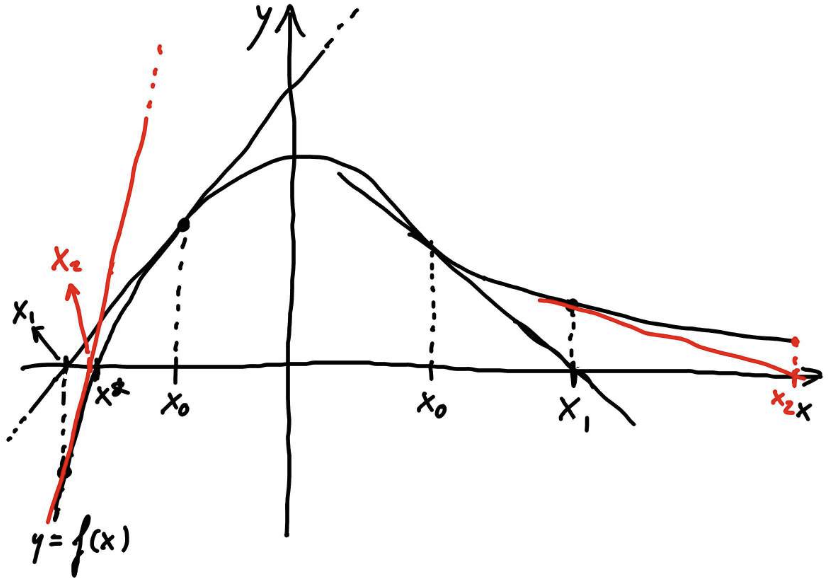
\includegraphics[width=0.75\textwidth]{immagini/EsemGeoConv.png}
	\caption{\label{fig:EsemGeoConv}Esempio dal punto di vista geometrico della convergenza.}
\end{figure}

Tramite la Figura \ref{fig:EsemGeoConv} è possibile osservare quanto segue: \begin{itemize}
	\item più le rette tangenti (le linee che toccano il grafico di $y=f(x)$) si avvicinano a $x^*$, più  il metodo converge ed è preciso;
	\item il problema di convergenza sorge se $x_0$ è scelto come nel primo quadrante perché i successivi calcoli ($x_1, x_2, \hdots$) si allontanano da $x^*$; quindi è necessario scegliere $x_0$ nell'intervallo locale della radice in base alla funzione.
\end{itemize}

\subsubsection{Studio della convergenza locale}
Questa Sezione è una formalizzazione della Figura \ref{fig:EsemGeoConv}.
Lo studio della convergenza locale in un contesto generale può essere formalizzata come segue: considerato un metodo iterativo per l'approssimazione di una radice, l'approssimazione della radice $x^*$ di $f$, è definita da
\begin{equation}\label{eq:funzIteraz}
	x_{i+1}=\Phi (x_i)\quad i=0,1,2,\hdots,
\end{equation}
con $\Phi (x_i)$ funzione d'iterazione, la quale caratterizza il metodo di iterazione generico \footnote{Tale funzione è una regola che fornisce una buona approssimazione applicando $\Phi$ a partire da $x_i$.}.

Affinché il metodo iterativo abbia senso, supposto che $x_i\rightarrow x^*$ per $i\rightarrow\infty$, è richiesto che $\boldsymbol{x^*}$ sia il \textbf{punto fisso} della funzione di iterazione $\boldsymbol{\Phi(x)}$, ovvero:
\begin{equation*}
	x^*=\Phi (x^*).
\end{equation*}

\begin{definition}[Funzione d'iterazione del metodo di Newton]
	Per il metodo di Newton la funzione di iterazione del metodo è
	\begin{equation}\label{eq:funzIterazNewton}
		\Phi (x)=x-\frac{f(x)}{f'(x)},
	\end{equation}
	quindi
	\begin{equation*}
		\Phi (x^*)=x^*-\frac{f(x^*)}{f'(x^*)}\overset{f(x^*)=0}{=}x^*.
	\end{equation*}
\end{definition}

Questo argomento permette di trattare le proprietà di convergenza del metodo iterativo, mediante lo studio delle proprietà di stabilità del punto fisso corrispondente della funzione di iterazione. La convergenza locale dei metodi può essere studiata mediante declinazioni del seguente teorema.

\begin{theorem}[\textbf{del punto fisso}]\label{th:puntofisso}
	\footnote{Slide 6 PDF lez9, PG 31-32.}
	Sia $\Phi(x)$ la funzione d'iterazione (\ref{eq:funzIteraz}) che definisce il metodo numerico. Supposto che $\exists\,\delta >0,\; 0\leq L<1$, costanti tali che:
	\begin{equation*}
		|\Phi (x)-\Phi (y)|\leq L|x-y| \quad\forall x,y \in I=(x^*-\delta,\, x^*+\delta),
	\end{equation*}
	allora:
	\begin{enumerate}
		\item $x^*$ è l'unico punto fisso di $\Phi$ in $I$;
		\item se $x_0 \in I\Rightarrow x_{i+1} = \Phi(x_i)\in I,\quad i=0,1,2,\hdots$;
		\item se $x_0\in I \Rightarrow \underset{{i\to\infty}}{\lim}{x_i}=x^*$. (proprietà più interessante)
	\end{enumerate}
\end{theorem}

\begin{proof}
	La dimostrazione avverrà per punti:
	\begin{enumerate}
		\item Per assurdo (è supposto che esistano due punti fissi): $\exists\, x^*,\, \overline{x}\in I: \Phi(x^*)=x^*,\, \Phi(\overline{x})=\overline{x}$. Poichè $x \neq \overline{x}$, segue:
		\begin{equation*}
			|x^*-\overline{x}|=|\Phi(x^*)-\Phi(\overline{x})|\overset{\footnotemark}{\leq}L|x^*-\overline{x}|<|x^*-\overline{x}| \Rightarrow\text{ Assurdo } (|x^*-\overline{x}|\overset{\footnotemark}{\nless}|x^*-\overline{x}|).
		\end{equation*}
		Quindi il punto fisso in $I$ è unico (e tale punto è $x^*$);
		\addtocounter{footnote}{-1}
		\footnotetext{Applicazione del teorema.}
		\stepcounter{footnote}
		\footnotetext{$|x^*-\overline{x}|$ non può essere minore di se stesso.}
		\item Per induzione: dato $x_0 \in I = (x^*-\delta,\, x^* + \delta)$ è supposto che $x_i\in I \iff |x_i-x^*|<\delta$, quindi è possibile dimostrare che $x_i\in I$ come segue:
		\begin{equation*}
			|x_{i+1}-x^*|=|\Phi(x_i)-\Phi(x^*)|\overset{\footnotemark}{\leq}L|x_i - x^*| < L\,\delta\overset{\footnotemark}{<}\delta\Rightarrow |x_{i+1}-x^*|<\delta\Rightarrow x_{i+1}\in I;
		\end{equation*}
		\item È necessario dimostrare
		\begin{equation*}
			\lim_{i\to\infty}{x_i}=x^*\iff \lim_{i\to\infty}{|x_i-x^*|}=0.
		\end{equation*}
		Ciò che interessa calcolare è $|x_i-x^*|$, ovvero l'errore:
		\begin{equation*}
			\begin{matrix}
				|x_i-x^*|&\overset{\footnotemark}{=}&|\Phi(x_{i-1})-\Phi(x^*)|&\leq& L|x_{i-1}-x^*|&=& L|\Phi(x_{i-2})-\Phi(x^*)|\\
				&\leq& L\cdot L |x_{i-2}-x^*|&=& L^2|x_{i-2}-x^*|&\leq& \hdots &\leq& L^i|x_0-x^*|\\
				&\Rightarrow& |x_i-x^*|&\leq& L^i|x_0-x^*|.
			\end{matrix}
		\end{equation*}
		Quindi è possibile dimostrare la tesi come segue:
		\begin{equation*}
			0\leq \underbrace{\lim_{i \to\infty}{|x_i-x^*|}}_{\footnotemark}\leq\lim_{i\to\infty}{L^i|x_0-x^*|}=0\Rightarrow \lim_{i\to\infty}{|x_i-x^*|}=0\Rightarrow\lim_{i\to\infty}{x_i=x^*}.
		\end{equation*}
	\end{enumerate}
\end{proof}

\addtocounter{footnote}{-4}
\footnotetext{Sfruttando le ipotesi del teorema.}

\stepcounter{footnote}
\footnotetext{$x_i,\, x^*\in I$.}

\stepcounter{footnote}
\footnotetext{$L<1$, quindi è valido ciò che segue.}

\stepcounter{footnote}
\footnotetext{$x_{i-1}, x^*\in I$ perché $x_0\in I$ e vale 2.}

\stepcounter{footnote}
\footnotetext{Limite calcolato con la disuguaglianza precedente.}

\noindent\footnote{Slide 1 PDF lez10, PG 32.} Inoltre, è possibile dimostrare che la funzione (\ref{eq:funzIterazNewton}) soddisfa le ipotesi del Teorema del punto fisso (Teorema \ref{th:puntofisso}), come segue: assumendo $f(x)\in C^{(2)}$ in un intorno di $x^*$, dove $x^*$ è la radice semplice di $f$ e definita $\Phi(x)\in C^{(1)}$ in un intorno di $x^*$ (come in (\ref{eq:funzIterazNewton})) con $\Phi'(x)=1-\frac{[f'(x)]^2-f(x)f''(x)}{[f'(x)]^2}$, allora
\begin{equation*}
	\Phi'(x^*)=1-\frac{[f'(x^*)]^2-f(x^*)f''(x^*)}{[f'(x^*)]^2}=1-\frac{[f'(x^*)]^2}{[f'(x^*)]^2}=1-1=0.
\end{equation*}
Quindi, $\Phi\in C^{(1)}\Rightarrow\Phi'\in C^{(0)}$ e $\Phi'(x^*)=0$.

Applicando la definizione di funzione continua\footnote{Definizione di funzione continua: $g$ è continua in $x^*$ s.se $\forall\varepsilon, \exists\,\delta>0:|g(x)-g(x^*)|<\varepsilon\quad\forall x\in I=(x^*-\delta,x^*+\delta)$.} a $\Phi=g$, $\varepsilon =L$ e fissato $0<L<1$:
\begin{equation*}
	\exists\,\delta>0:|\Phi'(x)-\Phi'(x^*)|<L \quad\forall x\in (x^*-\delta,x^*+\delta).
\end{equation*}


L'ipotesi è verificata con $L$ e $\delta$ scelte, utilizzando lo sviluppo di Taylor, in quanto
\begin{equation*}
	\begin{matrix}
		\forall x,y \in I=(x^*-\delta,\, x^*+\delta): |\Phi(x)-\Phi(y)| &\overset{\footnotemark}{=}& |\cancel{\Phi(x)}-\cancel{\Phi(x)}-\Phi'(\xi)(x-y)|  &\overset{\footnotemark}{=}& |\Phi'(\xi)(x-y)| \\
		&=& |\Phi'(\xi)||x-y| &<& L|x-y|\\
		&\Rightarrow&|\Phi(x)-\Phi(y)|&\leq& L|x-y|.
	\end{matrix}
\end{equation*}

\addtocounter{footnote}{-1}
\footnotetext{È necessario dimostrare che sia minore di $L|x-y|$. Inoltre, $\Phi(y)=\Phi(x)+\Phi(\xi)(x-y)$ con $\xi\in(x,y)\rightarrow\xi\in I$.}

\stepcounter{footnote}
\footnotetext{Approssimazione di $f(x)$ con sviluppo di Taylor.}

\begin{figure}
	\centering
	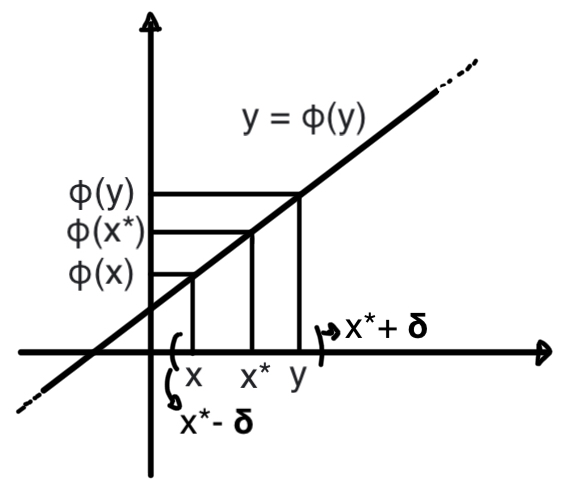
\includegraphics[width=0.5\textwidth]{immagini/TeoremaPuntoFisso.png}
	\caption{\label{fig:TeoremaPuntoFisso}Esempio del grafico di una funzione d'iterazione per il Teorema \ref{th:puntofisso}.}
\end{figure}

\subsubsection{Criteri d'arresto per il metodo di Newton (e non solo)}
\footnote{Slide 4 PDF lez10, PG 33.}
Gli argomenti trattati nella Sezione \ref{sec:critArresto}, riguardo la definizione di un criterio d'arresto basato sul controllo di $|f(x)|$ (ovvero $|f(x_i)|\leq|f'(x^*)|\, tolx$), sono applicati anche al caso del metodo di Newton (ed ai metodi quasi-Newton trattati in seguito). A causa della convergenza del metodo non è possibile determinare a priori il numero massimo di iterazioni entro le quali il criterio di accuratezza sulla approssimazione calcolata sarà soddisfatto. Dunque, in prossimità della radice $x^*$, nel caso di ordine di convergenza $p>1$,
\begin{equation}\label{eq:approxErroreNewton}
	|x_{i+1}-x_i|=|\underbrace{x_{i+1}-x^*}_{\text{$e_{i+1}$}}+\underbrace{x^*-x_i}_{\text{$e_{i}$}}|=|e_i-e_{i+1}|\overset{\footnotemark}{\approx}|e_i|.
\end{equation}
\footnotetext{$e_{i+1}\approx ce_i$. $\underset{i\to\infty}{\lim}\frac{|e_{i+1}|}{|e_i|^p}=c<\infty\Rightarrow |e_{i+1}|\approx c|e_i|^p\overset{p>1}{\Longrightarrow}e_{i+1}$ è trascurabile rispetto a $e_i$.}

Pertanto, un \textbf{criterio di arresto appropiato}, per metodi di \textbf{ordine di convergenza} $\boldsymbol{p>1}$ è del tipo
\begin{equation}\label{eq:critArrConvMag1}
	\boldsymbol{|x_{i+1}-x_i|\leq tolx}.
\end{equation}

Questo è dovuto al fatto che l'errore $|x^*-x_i|$ non è noto, quindi è necessario stimarlo, come in precedenza.

\begin{remark}[Criterio d'arresto per il metodo di Newton]
	Risulta essere sempre applicabile il seguente criterio d'arresto
	\begin{equation}\label{eq:critArrNewt}
		\boldsymbol{|f(x_i)|\leq |f'(x_i)|\cdot tolx}\equiv \frac{|f(x_i)|}{|f'(x_i)|}\leq tolx,
	\end{equation}
	il quale è ottenuto dalla Sezione \ref{sec:critArresto} tramite la disuguaglianza (\ref{eq:x_n_leq_tolx}) ($tolx$ ha lo stesso significato che ha in (\ref{eq:x_n_leq_tolx}
	)) .
\end{remark}

\begin{remark}[Criterio d'arresto ideale per il metodo di Newton]\footnote{Osservazione 2.3 PG 33, Slide 5 PDF lez10.}
	Oltre alla tolleranza sul massimo errore assoluto, $tolx$, è possibile utilizzare la tolleranza sull'errore relativo, $rtolx$ (o sull'accuratezza dell'approssimazione dello zero). In questo caso il controllo di arresto "ideale" diviene
	\begin{equation*}
		\frac{e_i}{tolx+rtolx|x^*|}\leq 1
	\end{equation*}
	e mediante le approssimazioni $x^*\approx x_{i+1}$ e $|e_i|\approx |x_{i+1}-x_i|$ il criterio da considerare è
	\begin{equation}\label{eq:critArrIdea}
		\boldsymbol{\frac{|x_{i+1}-x_i|}{tolx+rtolx|x_{i+1}|}\leq 1}.
	\end{equation}
	dove la disuguaglianza $e_i\leq tolx+rtolx|x^*|$ può essere rappresentata come
	\begin{equation*}
		\boldsymbol{\frac{1}{2}|e_i|\leq tolx} \wedge \frac{1}{2}|e_i|\leq rtolx|x^*| \iff \boldsymbol{\frac{1}{2}\frac{|e_i|}{x^*}\leq rtolx}
	\end{equation*}
	permettono di dividere in due il controllo (mediante ciò che è in grassetto). È spesso considerata la scelta $rtolx=tolx$, trasformando il criterio d'arresto (\ref{eq:critArrIdea}) in
	\begin{equation*}
		\frac{|x_{i+1}-x_i|}{1+|x_{i+1}|}\leq tolx.
	\end{equation*}
\end{remark}

Nel caso in cui la convergenza sia lineare (ovvero l'ordine di convergenza è $p=1$), il criterio d'arresto (\ref{eq:critArrConvMag1}) può essere modificato nel seguente (come \ref{eq:critArrIdea}), date (\ref{eq:limite_errore_metodo_convergente})-(\ref{eq:limOrdConv}) e (\ref{eq:limCostanteAsistotica})):

\begin{equation}\label{eq:approxErroreNewtonBis}
	|x_{i+1}-x_i|=|e_{i+1}-e_i|=|e_i-\underbrace{e_{i+1}}_\text{$c\cdot e_i$}|\approx |e_i|(1-c)\Rightarrow |e_i|\approx\frac{|x_{i+1}-x_i|}{\underset{\footnotemark}{(1-c)}}.
\end{equation}
\footnotetext{Senza valore assoluto perché, per definizione di convergenza, i metodi convergenti hanno costante asintotica $c$ minore di 1.}

Se $c$ non è nota (nel caso del metodo di bisezione è $c=\frac{1}{2}$), è possibile, tramite (\ref{eq:approxErroreNewtonBis}), la seguente stima della costante asintotica c:
\begin{equation*}
	\boldsymbol{\frac{|x_{i+1}-x_i|}{|x_i-x_{i-1}|}\approx}\frac{\cancel{|e_{i-1}|}\,c\,\cancel{(1-c)}}{\cancel{|e_{i-1}|}\cancel{(1-c)}}=\boldsymbol c,
\end{equation*}
la quale è ottenuta tramite $i$ iterazioni del tipo
\begin{equation*}
	\begin{matrix}
		i=0 &:& |x_1-x_0|&\approx& |e_0|(1-c);\\
		i=1 &:& |x_2-x_1|&\approx&|e_i|(1-c)&\overset{\footnotemark}{\approx}&|e_0|\, c\, (1-c);\\
		\vdots & & \vdots & & \vdots \\
		i &:&|x_i-x_{i-1}|&\approx& |e_{i-1}|(1-c);\\
		i+1 &:&|x_{i+1}-x_i|&\approx& |e_i|(1-c) &=& |e_{i-1}|\, c\, (1-c);
	\end{matrix}
\end{equation*}
per renderla più precisa. Tale stima è utile per avere una buona  approssimazione dell'errore. Pertanto, è necessario considerare il costo computazionale delle $i$ iterazioni (sono necessarie almeno due iterazioni).
\footnotetext{$e_{i+1}\approx c\cdot e_i$.}

\subsubsection{Caso delle radici multiple}
\footnote{Slide 1-3 PDF lez11, PG 34-36.}
Nel caso in cui la molteplicità di $x^*$ sia $m>1$, è noto che il problema di determinare le radici sia malcondizionato. Inoltre, è noto che il metodo di Newton risulti essere solo lineare. Tuttavia, è possibile modificare tale metodo per ripristinare la convergenza quadratica, distinguendo i seguenti casi.

\subsubsubsection{Molteplicità \texorpdfstring{$\boldsymbol{m>1}$}{m>1} nota}
Avere $m$ nota non è una caratteristica banale. Applicando l'Osservazione \ref{rem:formaF}, per semplicità, al metodo di Newton, per determinare la radice (\ref{eq:approxNewton}), allora, è ottenuta
\begin{equation*}
	x_{i+1}=x_i-\frac{x_i-x^*}{m}, \quad i=0,1,2,\hdots.
\end{equation*}
Pertanto, il metodo di Newton è modificato come segue:
\begin{equation}\label{eq:approxNewtonMod}
	x_{i+1}=x_i-m\frac{f(x_i)}{f'(x_i)}, \quad i=0,1,2,\hdots,
\end{equation}
ripristinando la convergenza quadratica del metodo, qualora converga verso una radice di molteplicità esatta $m$.

\paragraph{Nota:} Saranno presenti riferimenti a questo paragrafo ed a (\ref{eq:approxNewtonMod}) come metodo di Newton modificato.

\paragraph{Convergenza:} Nel caso generale la \textbf{convergenza} rimane \textbf{quadratica}.

\subsubsection{Molteplicità \texorpdfstring{$\boldsymbol{m>1}$}{m>1} ignota}
In questo caso il metodo di Newton converge linearmente ($p=1$), quindi (da (\ref{eq:limOrdConv}))
\begin{equation*}
	\underset{i\to\infty}{\lim}{\frac{|e_{i+1}|}{|e_i|}} = c<\infty.
\end{equation*}

Allora, per $i$ sufficientemente grande:
\begin{equation*}
	\begin{matrix}
		\boldsymbol{\frac{|e_{i+1}|}{e_i}\approx c}&\Rightarrow&
		\begin{matrix}
			e_i &\approx& c\cdot e_{i-1}\\
			e_{i+1}&\approx& c\cdot e_i
		\end{matrix}\\
		&\Rightarrow& e_i &\approx& \frac{e_{i+1}}{c}\\
		&\overset{\footnotemark}{\Rightarrow}& e_i^2&=&e_i\,e_i&\approx&\cancel{c}\cdot e_{i-1}\cdot \frac{e_{i+1}}{\cancel{c}}&=&e_{i-1}\cdot e_{i+1}\\
		&\boldsymbol\Rightarrow&\boldsymbol{e_i^2}&\boldsymbol\approx& \boldsymbol{e_{i-1}\cdot e_{i+1}}.
	\end{matrix}
\end{equation*}
\footnotetext{Dalle due relazioni (approssimazioni) è possibile ottenere ciò che segue.}

È possibile riscrivere la precedente approssimazione, l'ultima implicazione, come
\begin{center}
	$\underbrace{(x_i-x^*)^2}_{\text{$e_i^2$}}\approx\underbrace{(x_{i-1}-x^*)}_{\text{$e_{i-1}$}}\underbrace{(x_{i+1}-x^*)}_{\text{$e_{i+1}$}}$ 
\end{center}
e da questa segue che
\begin{equation*}
	\begin{matrix}
		x_i^2-2x_i x^*+\cancel{(x^*)^2}&\approx& x_{i-1} x_{i+1}-x_{i-1} x^* - x_{i+1} x^*+\cancel{(x^*)^2}\\
		&\rightarrow&-2x_i x^*+x_{i-1} x^*+x_{i+1}x^*&\approx&-x_i^2+x_{i-1} x_{i+1}\\
		&\rightarrow&(-2x_i+x_{i-1}+x_{i+1})x^* &\approx& -x_i^2+x_{i-1} x_{i+1}.
	\end{matrix}
\end{equation*}

Da quest'ultima approssimazione è possibile la seguente approssimazione della radice:
\begin{equation}\label{eq:approxAitken}
	x^*\approx x_i^*\equiv\frac{x_i^2-x_{i-1}\cdot x_{i+1}}{2x_i-x_{i-1}-x_{i+1}},
\end{equation}
dove $x_i^*$ rappresenta l'approssimazione di $x^*$ al passo $i-$esimo.

\begin{algorithm}
	\caption{Implementazione efficiente del metodo di Newton.}\label{alg:polNewt}
	\begin{lstlisting}[style=Matlab-editor]
		function x = newton(f, f1, x0, tol, itmax)
		%   
		%   x = newton(f, f1, x0, tol, itmax)
		%
		%   Metodo di Newton per la ricerca della radice di una funzione
		%
		% Input:
		%   f   -   function che implementa f(x);
		%   f1  -   function che implementa f'(x);
		%   x0  -   punto iniziale:
		%   tol -   tolleranza richiesta (default 1e-12);
		%   itmax   - numero massimo di iterazioni (default 1000);
		% Output:
		%   x   -   soluzione approssimata.
		%
		% Dalla riga successuva fino a x = x0 sono controlli strutturali.
		if nargin < 5
		itmax=1000;
		else
		if itmax < 1, error('itmax errato'); end
		end
		if nargin < 4 
		tol = 1e-12;
		else
		if tol < 0, error('tolleranza negativa'); end
		tol = max(tol, 10*eps);
		end
		if nargin < 3,  error('numero argomenti di ingresso errato'); end
		x = x0;
		for i = 1 : itmax
		xold = x;
		fx = feval(f,x);
		f1x = feval(f1, x);
		if f1x == 0, error('il metodo non converge'); end
		x = x - fx/f1x;
		err = abs(x-xold);
		if err <= tol, break; end
		end
		if err > tol, warning('tolleranza richiesta non soddifatta'), end
		return
	\end{lstlisting}
\end{algorithm}

\subsection{Metodo di Aitken}
\footnote{Slide 4-5 PDF lez11, PG 36-37.}
Il metodo utilizza una procedura a due livelli:
\begin{enumerate}
	\item Vengono eseguiti due passi del metodo di Newton (\ref{eq:approxNewton}): 
	\begin{itemize}
		\item $x_{i-1}=x_{i-1}^*$;
		\item $x_i=x_{i-1}-\frac{f(x_{i-1})}{f'(x_{i-1})}$;
		\item $x_{i+1}=x_i-\frac{f(x_i)}{f'(x_i)}$;
	\end{itemize}
	\item Passo di Aitken: esecuzione del passo (\ref{eq:approxAitken}) di accelerazione, approssimare al meglio la radice. Questo passo fornirà il nuovo punto iniziale per il livello interno.
\end{enumerate}
La successione $\{x_i^*\}_{i=1,2,\hdots}$ generata con Aitken \underline{converge quadraticamente} verso $x^*$.
\paragraph{Costo computazionale} Pertanto, il prezzo di avere un'iterazione a due livelli è pagato con un costo computazionale doppio rispetto al classico Newton, ad ogni iterazione è applicato Newton due volte (per le quali sono necessarie le valutazioni di $f$ e $f'$).

\begin{algorithm}
	\caption{Implementazione metodo di Aitken.}\label{alg:metAit}
	\begin{lstlisting}[style=Matlab-editor]
		function x = aitken(f, f1, x, tolx, itmax)
		x = x0;
		for i = 1 : itmax
		x0 = x;
		fx = feval(f, x0);
		f1x = feval(f1, x0);
		x1 = x0 - fx/f1x;
		fx = feval(f, x1);
		f1x = feval(f1, x1);
		x = x1 - fx/f1x;
		x = (x*x0 - x1^2)/(x - 2*x1 + x0);
		if abs(x-x0) <= tolx, break, end
		end
		if abs(x-x0) > tolx, warning('il metodo non converge'), end
	\end{lstlisting}
\end{algorithm}

\subsection{Metodi quasi-Newton}
\footnote{Slide 6-10 PDF 11, PG 37-40.}
È possibile ridurre il costo di ogni iterazione del tipo (\ref{eq:approxNewton}) attraverso un'approssimazione di $f'(x_i)$. I metodi in questa Sezione, variazioni del metodo di Newton, calcolano $x_{i+1}$ come segue:
\begin{equation}\label{eq:approxQuasiNewton}
	x_{i+1}=x_i-\frac{f(x_i)}{\varphi_i}, \quad i=0,1,2,\hdots, \quad\varphi_i\approx f'(x_i).
\end{equation}

\subsubsection{Metodo delle corde}
È assunto che $f(x)$ sia sufficientemente regolare ed è presupposto che la derivata vari di poco in prossimità della radice.
Pertanto, se $x_0$ è vicino alla radice, allora è possibile approssimare $f'$ come
\begin{equation*}
	f'(x_i)\approx f'(x_0)\equiv\varphi_i,\; i=0,1,2,\hdots.
\end{equation*}
In questo modo è ottenuta l'iterazione 
\begin{equation}\label{eq:approxCorde}
	x_{i+1}=x_i-\frac{f(x_i)}{f'(x_0)}, \quad i=0,1,2,\hdots,
\end{equation}
la quale definisce il metodo delle corde.

È necessario notare che l'approssimazione della derivata sia una costante (ovvero $f'(x_0)$).

\paragraph{Costo computazionale:}\footnote{Il costo computazionale è considerato per iterazione.} 1 valutazione funzionale ($f(x_i)$).
\paragraph{Covergenza:}Si, locale.
\paragraph{Ordine di convergenza:} È lineare ($p = 1$) qualsiasi sia la molteplicità della radice.

Il metodo è utilizzato per la risoluzione di sistemi lineari per il basso costo di computazionale.

\subsubsection{Metodo delle secanti}\label{sssec:metodo_secanti}
\footnote{Slide 7-10 PDF lez11.}
Supposto siano già calcolati $x_{i-1}$ ed $x_i$, allora $f(x)\approx f(x_i)+(x-x_i)f'(x_i)$. La derivata può essere approssimata come 
\begin{equation*}
	f'(x_i)\approx\frac{f(x)-f(x_{i})}{x-x_i}\overset{x=x_{i-1}}{\Longrightarrow}f'(x_i)\approx\frac{f(x_i)-f(x_{i-1})}{x_i-x_{i-1}}\equiv\varphi_i.
\end{equation*}

L'iterazione (\ref{eq:approxQuasiNewton}) diviene
\begin{equation}\label{eq:approxSecanti}
	\boldsymbol{x_{i+1}=x_i-\frac{f(x_i)(x_i-x_{i-1})}{f(x_i)-f(x_{i-1})}}=\frac{f(x_i)\,x_{i-1} - f(x_{i-1})\,x_i}{f(x_i)-f(x_{i-1})}, \quad i=1,2,\hdots,
\end{equation}
con $x_0$ ed $x_1$ approssimazioni iniziali assegnate (sono richiesti per il calcolo di $x_2$). Assegnato $x_0$ è possibile calcolare $x_1$, tramite il metodo di Newton, come $x_1=x_0-\frac{f(x_0)}{f'(x_0)}$.

\begin{figure}
	\centering
	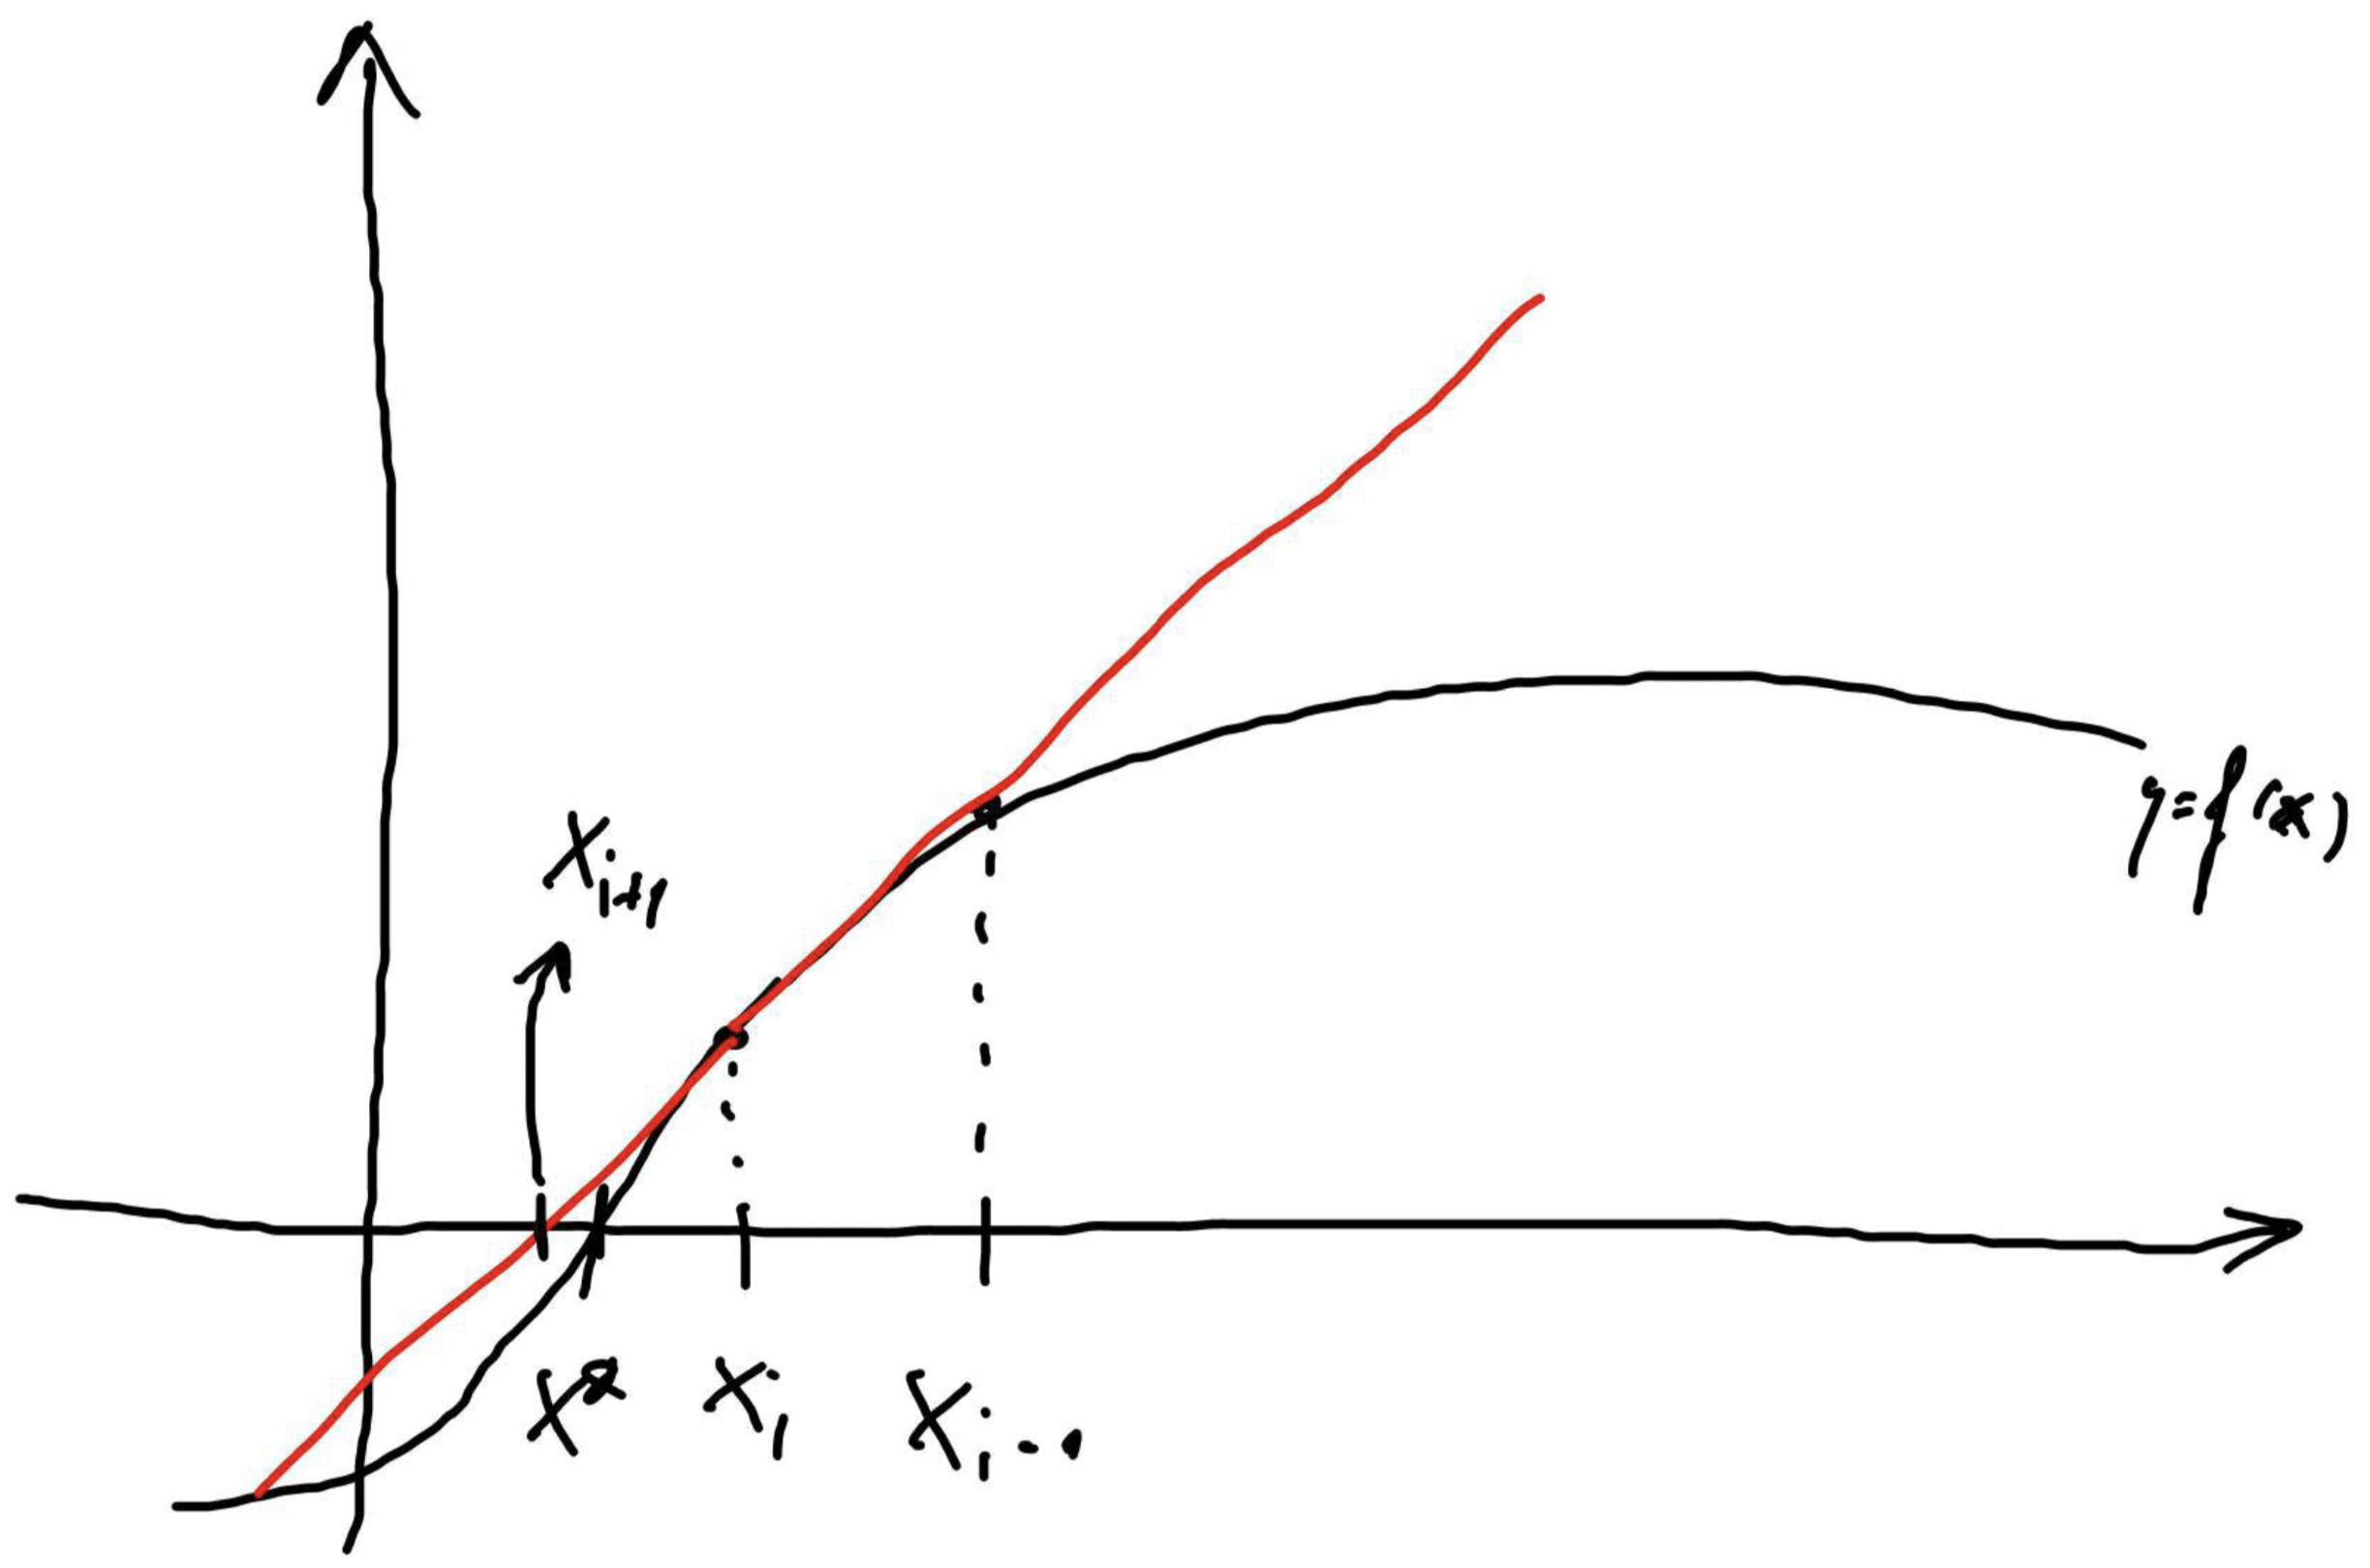
\includegraphics[width=0.5\textwidth]{immagini/GraficoSecanti.png}
	\caption{\label{fig:GraficoSecanti} Metodo delle secanti (\ref{eq:approxSecanti}). La linea rossa dovrebbe passare per $x_{i+1},\; x_i\; e\; x_{i-1}$.}
\end{figure}

\paragraph{Costo computazionale:}\footnote{Slide 9 PDF lez11.}
L'approssimazione (\ref{eq:approxSecanti}) richiede una valutazione funzionale per iterazione, in quanto $f(x_{i-1})$ è calcolato al passo $i-1$. La prima iterazione ne richiede due, ma sono trascurabili.

\paragraph{Convergenza:}\footnote{Slide 10 PDF lez11.} locale. Inoltre, il metodo delle secanti è superlineare, ovvero: la successione delle approssimazioni converge alla radice della funzione con un tasso di convergenza maggiore rispetto al metodo delle tangenti e al metodo della bisezione, ma minore rispetto al metodo di Newton.

\paragraph{Ordine di convergenza:} $p = \frac{\sqrt{5}+1}{2}\approx 1.618$ per radici semplici. Anche se l'ordine di convergenza è minore rispetto a quello del metodo di Newton è preferibile a quest'ultimo, in quanto non viene effettuata una valutazione della derivata ad ogni iterazione.

\begin{remark}
	Nella conversione dei precenti metodi in algoritmi è buona norma eseguire controlli sul demominatore, affinchè non siano svolte divisioni per 0. Nel caso dell'approssimazione di radici multiple, mediante il metodo di Newton modificato o il metodo di accelerazione Aitken, quando la derivata si annulla ed il valore della funzione è molto piccolo, significa che è stata raggiunta la migliore approssimazione possibile della soluzione.
\end{remark}

\begin{algorithm}
	\caption{Implementazione del metodo delle secanti.}\label{alg:metodo_secanti}
	\begin{lstlisting}[style=Matlab-editor]
		function xstar = secanti(fun, x0, x1, tol, itmax)
		% 
		% xstar = secanti(f, x0, x1, tol, itmax)
		% 
		% Calcola una approssimazione della radice di f(x) con tolleranza tol.
		% 
		% Input:
		%     f - identidicatore della function che implementa f(x);
		%     x0, x1 - punti iniziali;
		%     tol - accuratezza richiesta (default tol = 10^(-6));
		%     itmax - numero massimo di iterazioni (default itmax = 1000).
		% 
		% Output:
		%     xstar - approssimazione della soluzione.
		if nargin < 3
			error('numero di argomenti in ingresso errato')
		elseif nargin == 3
			tol =1e-6; itmax = 1000;
		elseif nargin == 4
			itmax = 1000;
		end
		
		if tol <= 0, error('tolleranza errata'); end
		if itmax <= 0, error('itmax errato'); end
		
		f0 = feval(fun, x0);
		f1 = feval(fun, x1);
		
		for i = 1:itmax
			if f0 == f1 && f1 ~= 0
				error('il metodo non converge');
			end
			
			xstar = (x0*f1 - x1*f0)/(f1 - f0);
			delta = abs(xstar - x1);
			
			if delta <= tol * (1 + abs(xstar))
				break
			elseif i < itmax
				x0 = x1; xstar = x1;
				f0 = f1; f1 = feval(fun,x1);
			end
		end
		
		if delta > tol * (1+abs(xstar))
			warning('accuratezza richiesta non raggiunta');
		end
		return
	\end{lstlisting}
\end{algorithm}